\newpage
\section{Results and Discussion}\label{sec:results}

All values are medians of \Reps{} measured samples; error bars and bracketed ranges are the IQR. Bold entries in the tables mark the best implementation at each thread count. The complete tables for every experiment are in Appendix~\ref{app:tables}. Explanations that rely on the hardware or the scheduler, rather than on a measurement, are marked as hypotheses.

\subsection{Mutex locks with a fixed total amount of work}\label{sec:res-locks}

Figure~\ref{fig:locks-fixed} shows the program time of the statement's workload for a fixed total of $K=20000$ iterations, so that the total work does not change with $P$.

\begin{figure}[H]
\centering
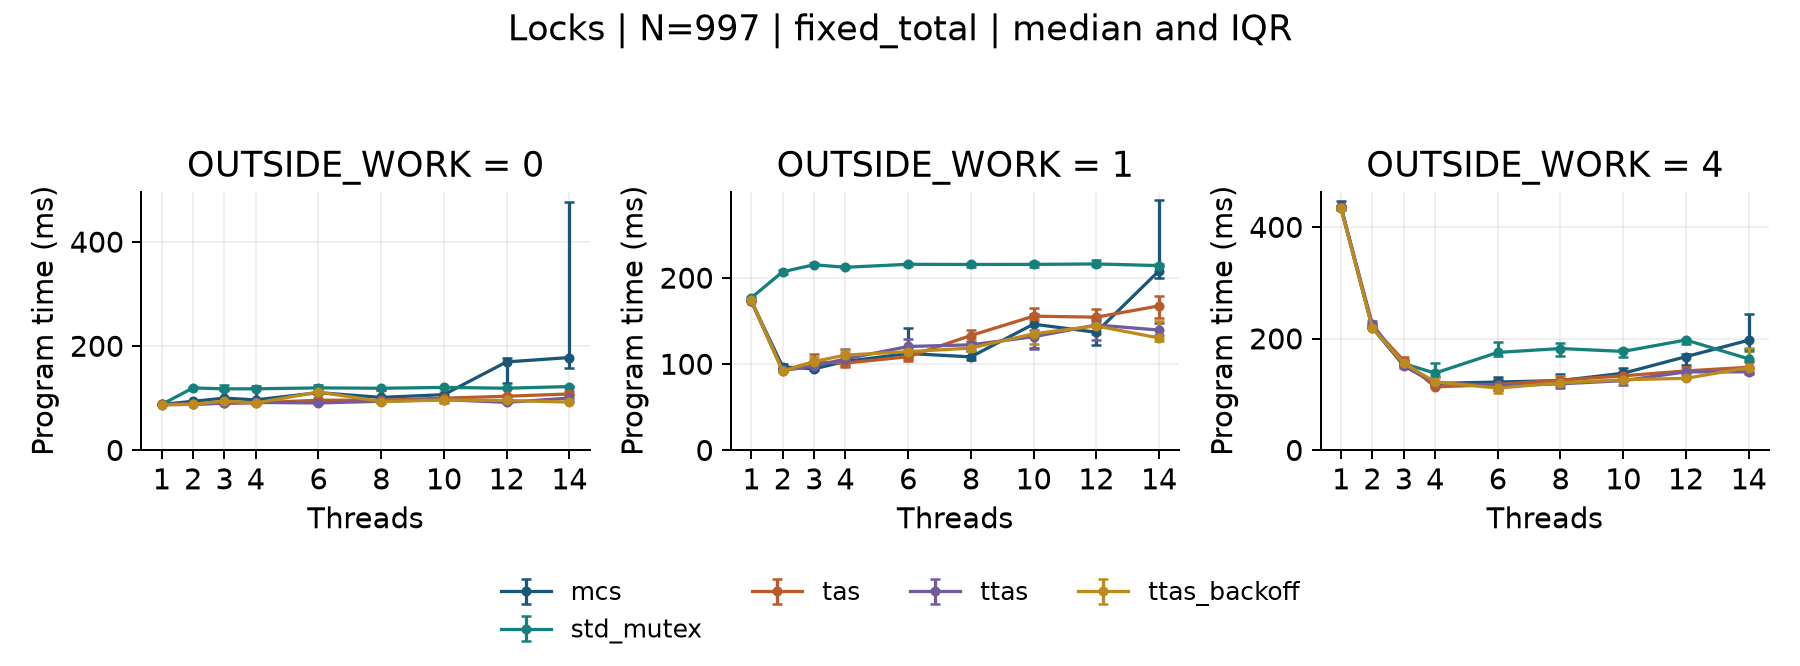
\includegraphics[width=\textwidth]{figures/locks_fixed_total.png}
\caption{Lock program time, fixed total $K=20000$, $N=997$, for $W=0,1,4$ (median and IQR).}\label{fig:locks-fixed}
\end{figure}

\textbf{All work inside the lock ($W=0$).} Equation~\eqref{eq:amdahl} allows no speedup, so the best a lock can do is to keep $T(P)$ at $T(1)\approx87.6$~ms (Table~\ref{tab:locks-fixed-w0}). TAS, TTAS and TTAS-backoff stay between 87 and 112~ms up to $P=14$. \texttt{std::mutex} rises to 119~ms as soon as $P=2$ and then stays flat. MCS stays within 26\% of $T(1)$ up to $P=10$ and climbs to 169--178~ms at $P=12$--14.

\begin{table}[H]
\centering
\footnotesize
\setlength{\tabcolsep}{3pt}
\caption{Median program time (ms), fixed total $K=20000$, $N=997$, $W=0$. Bold: fastest at each $P$.}\label{tab:locks-fixed-w0}
\begin{tabular}{|>{\raggedright\arraybackslash}p{\dimexpr 0.200\textwidth-2\tabcolsep-\arrayrulewidth\relax}|>{\raggedleft\arraybackslash}p{\dimexpr 0.088\textwidth-2\tabcolsep-\arrayrulewidth\relax}|>{\raggedleft\arraybackslash}p{\dimexpr 0.088\textwidth-2\tabcolsep-\arrayrulewidth\relax}|>{\raggedleft\arraybackslash}p{\dimexpr 0.088\textwidth-2\tabcolsep-\arrayrulewidth\relax}|>{\raggedleft\arraybackslash}p{\dimexpr 0.088\textwidth-2\tabcolsep-\arrayrulewidth\relax}|>{\raggedleft\arraybackslash}p{\dimexpr 0.088\textwidth-2\tabcolsep-\arrayrulewidth\relax}|>{\raggedleft\arraybackslash}p{\dimexpr 0.088\textwidth-2\tabcolsep-\arrayrulewidth\relax}|>{\raggedleft\arraybackslash}p{\dimexpr 0.088\textwidth-2\tabcolsep-\arrayrulewidth\relax}|>{\raggedleft\arraybackslash}p{\dimexpr 0.088\textwidth-2\tabcolsep-\arrayrulewidth\relax}|>{\raggedleft\arraybackslash}p{\dimexpr 0.088\textwidth-2\tabcolsep-\arrayrulewidth\relax}|}
\hline
\textbf{Lock (ms)} & \textbf{P=1} & \textbf{P=2} & \textbf{P=3} & \textbf{P=4} & \textbf{P=6} & \textbf{P=8} & \textbf{P=10} & \textbf{P=12} & \textbf{P=14} \\ \hline
\texttt{tas} & 87.5 & 88.5 & 90.1 & 90.7 & 95.7 & 95.6 & 99.6 & 103.4 & 107.7 \\ \hline
\texttt{ttas} & 87.3 & \textbf{87.7} & \textbf{90.0} & 91.5 & \textbf{90.4} & 93.7 & 96.9 & \textbf{91.6} & 99.8 \\ \hline
\texttt{ttas\_backoff} & \textbf{86.8} & 87.9 & 94.1 & \textbf{90.3} & 111.5 & \textbf{93.1} & \textbf{96.1} & 95.3 & \textbf{92.1} \\ \hline
\texttt{mcs} & 87.6 & 93.6 & 99.7 & 96.3 & 110.2 & 101.1 & 106.4 & 169.3 & 177.6 \\ \hline
\texttt{std\_mutex} & 87.6 & 119.3 & 117.6 & 117.6 & 119.4 & 118.7 & 120.3 & 118.8 & 121.9 \\ \hline
\end{tabular}
\end{table}


\textbf{Work outside the lock ($W>0$).} Now the threads can overlap their outside calls, and Table~\ref{tab:speedup-w4} shows how close each lock comes to the bound $S\le W+1$. At $W=1$ the spinlocks reach 1.9$\times$ at $P=2$, close to the bound of 2. At $W=4$ (bound 5) the best speedup is 3.9$\times$ (TTAS-backoff, $P=6$), and at $W=8$ (bound 9) it is 5.6$\times$ (TAS, $P=12$; Table~\ref{tab:speedup-w8}). The gap to the bound grows with $W$ because more threads are needed to approach it, and more threads contend for the lock at every release.

\begin{table}[H]
\centering
\footnotesize
\setlength{\tabcolsep}{3pt}
\caption{Speedup $S(P)=T(1)/T(P)$, fixed total, $N=997$, $W=4$ (Amdahl bound 5$\times$). Bold: highest at each $P$.}\label{tab:speedup-w4}
\begin{tabular}{|>{\raggedright\arraybackslash}p{\dimexpr 0.200\textwidth-2\tabcolsep-\arrayrulewidth\relax}|>{\raggedleft\arraybackslash}p{\dimexpr 0.099\textwidth-2\tabcolsep-\arrayrulewidth\relax}|>{\raggedleft\arraybackslash}p{\dimexpr 0.099\textwidth-2\tabcolsep-\arrayrulewidth\relax}|>{\raggedleft\arraybackslash}p{\dimexpr 0.099\textwidth-2\tabcolsep-\arrayrulewidth\relax}|>{\raggedleft\arraybackslash}p{\dimexpr 0.099\textwidth-2\tabcolsep-\arrayrulewidth\relax}|>{\raggedleft\arraybackslash}p{\dimexpr 0.099\textwidth-2\tabcolsep-\arrayrulewidth\relax}|>{\raggedleft\arraybackslash}p{\dimexpr 0.099\textwidth-2\tabcolsep-\arrayrulewidth\relax}|>{\raggedleft\arraybackslash}p{\dimexpr 0.099\textwidth-2\tabcolsep-\arrayrulewidth\relax}|>{\raggedleft\arraybackslash}p{\dimexpr 0.099\textwidth-2\tabcolsep-\arrayrulewidth\relax}|}
\hline
\textbf{Lock} & \textbf{P=2} & \textbf{P=3} & \textbf{P=4} & \textbf{P=6} & \textbf{P=8} & \textbf{P=10} & \textbf{P=12} & \textbf{P=14} \\ \hline
\texttt{tas} & 1.97 & 2.72 & \textbf{3.84} & 3.71 & 3.47 & 3.27 & 3.07 & 2.93 \\ \hline
\texttt{ttas} & 1.92 & 2.88 & 3.60 & 3.77 & \textbf{3.66} & \textbf{3.49} & 3.10 & \textbf{3.10} \\ \hline
\texttt{ttas\_backoff} & 1.98 & 2.79 & 3.55 & \textbf{3.90} & 3.60 & 3.44 & \textbf{3.37} & 2.93 \\ \hline
\texttt{mcs} & \textbf{1.99} & \textbf{2.88} & 3.66 & 3.58 & 3.51 & 3.17 & 2.61 & 2.22 \\ \hline
\texttt{std\_mutex} & 1.97 & 2.80 & 3.14 & 2.48 & 2.38 & 2.45 & 2.20 & 2.65 \\ \hline
\end{tabular}
\end{table}

\begin{table}[H]
\centering
\footnotesize
\setlength{\tabcolsep}{3pt}
\caption{Speedup $S(P)=T(1)/T(P)$, fixed total, $N=997$, $W=8$ (Amdahl bound 9$\times$). Bold: highest at each $P$.}\label{tab:speedup-w8}
\begin{tabular}{|>{\raggedright\arraybackslash}p{\dimexpr 0.200\textwidth-2\tabcolsep-\arrayrulewidth\relax}|>{\raggedleft\arraybackslash}p{\dimexpr 0.099\textwidth-2\tabcolsep-\arrayrulewidth\relax}|>{\raggedleft\arraybackslash}p{\dimexpr 0.099\textwidth-2\tabcolsep-\arrayrulewidth\relax}|>{\raggedleft\arraybackslash}p{\dimexpr 0.099\textwidth-2\tabcolsep-\arrayrulewidth\relax}|>{\raggedleft\arraybackslash}p{\dimexpr 0.099\textwidth-2\tabcolsep-\arrayrulewidth\relax}|>{\raggedleft\arraybackslash}p{\dimexpr 0.099\textwidth-2\tabcolsep-\arrayrulewidth\relax}|>{\raggedleft\arraybackslash}p{\dimexpr 0.099\textwidth-2\tabcolsep-\arrayrulewidth\relax}|>{\raggedleft\arraybackslash}p{\dimexpr 0.099\textwidth-2\tabcolsep-\arrayrulewidth\relax}|>{\raggedleft\arraybackslash}p{\dimexpr 0.099\textwidth-2\tabcolsep-\arrayrulewidth\relax}|}
\hline
\textbf{Lock} & \textbf{P=2} & \textbf{P=3} & \textbf{P=4} & \textbf{P=6} & \textbf{P=8} & \textbf{P=10} & \textbf{P=12} & \textbf{P=14} \\ \hline
\texttt{tas} & 1.96 & \textbf{2.91} & \textbf{3.88} & 4.30 & 4.88 & \textbf{5.41} & \textbf{5.65} & 4.95 \\ \hline
\texttt{ttas} & 1.95 & 2.90 & 3.69 & 3.91 & \textbf{5.20} & 5.33 & 5.57 & \textbf{5.45} \\ \hline
\texttt{ttas\_backoff} & 1.95 & 2.83 & 3.39 & 4.36 & 4.86 & 5.38 & 5.41 & 5.41 \\ \hline
\texttt{mcs} & 1.97 & 2.89 & 3.59 & \textbf{5.08} & 5.02 & 5.29 & 4.58 & 3.74 \\ \hline
\texttt{std\_mutex} & \textbf{1.99} & 2.90 & 3.67 & 3.29 & 3.20 & 3.26 & 3.22 & 3.15 \\ \hline
\end{tabular}
\end{table}


\textbf{Beyond 6 to 10 threads} every lock gets slower again (Figure~\ref{fig:locks-fixed}, right). More waiters compete for the lock's cache line at each release. In addition, the laptop has only 6 performance cores, so higher $P$ places threads on the efficiency cores and on Hyper-Threading siblings, which run the primality loop more slowly. This placement explanation is a hypothesis consistent with the data, not a measured scheduler trace.

\subsection{Cost of passing the lock}\label{sec:res-outside}

In per-thread mode every thread performs $I=5000$ iterations, so the total work grows with $P$ (Figure~\ref{fig:locks-per-thread}); this is the statement's program as given. With $W=0$ all of that work is serial, so $T(P)\ge P\cdot T(1)$, and the ratio $T(P)/(P\cdot T(1))$ measures what each lock adds on top of the serial work, mainly the cost of passing ownership from one thread to the next. Computed from Table~\ref{tab:locks-per-thread-w0}, the ratio at $P=14$ is 1.03 for TTAS, 1.06 for TTAS-backoff, 1.18 for TAS, 1.34 for \texttt{std::mutex} and 1.64 for MCS. \texttt{std::mutex} costs 1.33--1.35 at every $P$ from 2 to 14, a fixed price per handoff; TAS and MCS start near 1.0 and grow with $P$, which is the signature of contention.

\begin{figure}[H]
\centering
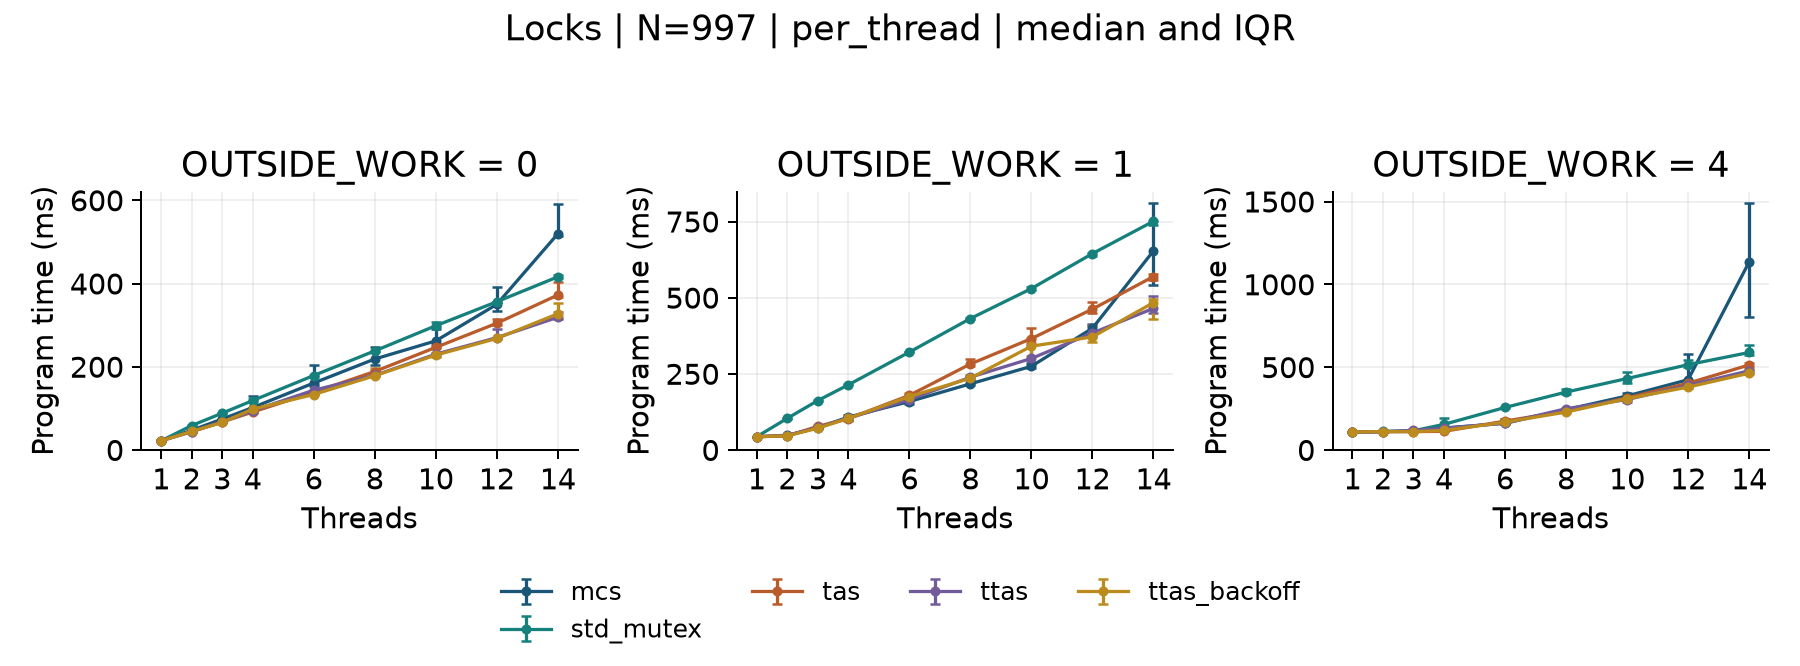
\includegraphics[width=\textwidth]{figures/locks_per_thread.png}
\caption{Lock program time, per-thread $I=5000$, $N=997$, for $W=0,1,4$; total work grows with $P$.}\label{fig:locks-per-thread}
\end{figure}

\subsection{Length of the critical section}\label{sec:res-sensitivity}

Figure~\ref{fig:locks-sens} changes $N$ to make each critical section about ten times shorter ($N=97$) or longer ($N=10007$). With short critical sections the lock changes owner very often. TAS then degrades from 82~ms at $P=1$ to 244~ms at $P=14$, because every waiter keeps executing \texttt{test\_and\_set} on the shared line, while TTAS, which waits with plain reads, stays at 89--106~ms for $P=2$--14 (Table~\ref{tab:sens-n97-w0}). This is the difference between TAS and TTAS that the slides predict, and it appears only when handoffs are frequent: with long critical sections all locks stay within 87--115~ms except MCS at $P=14$ (225~ms).

\begin{figure}[H]
\centering
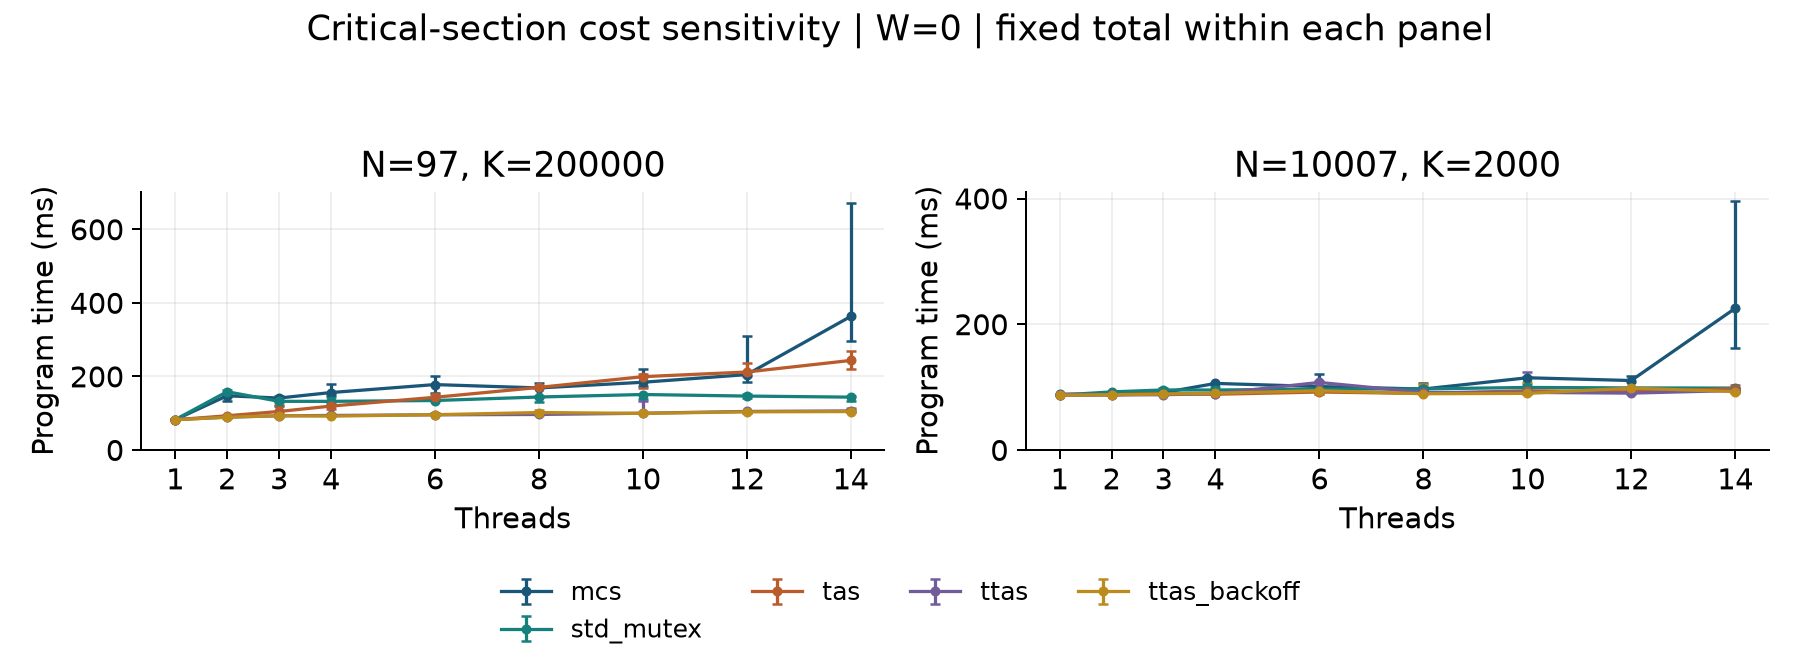
\includegraphics[width=\textwidth]{figures/locks_sensitivity.png}
\caption{Short ($N=97$, $K=200000$) and long ($N=10007$, $K=2000$) critical sections, $W=0$.}\label{fig:locks-sens}
\end{figure}

\subsection{Saturating every logical CPU}\label{sec:res-saturation}

Table~\ref{tab:saturation-locks} adds $P=15$ and 16. TAS, TTAS, TTAS-backoff and \texttt{std::mutex} stay at 91--122~ms at every $P$. MCS rises from 116~ms at $P=12$ to 333~ms at $P=15$ and 2468~ms at $P=16$, and its third quartile at $P=16$ is 61~s (Table~\ref{tab:saturation-locks-q3}); single runs at $P=16$ ranged from 0.18~s to 85~s. In the main run, one MCS warm-up at $P=14$ also exceeded 60~s.

\begin{table}[H]
\centering
\footnotesize
\setlength{\tabcolsep}{3pt}
\caption{Saturation run: median program time (ms), $N=997$, $W=0$, $K=20000$, five measured runs. Bold: fastest at each $P$.}\label{tab:saturation-locks}
\begin{tabular}{|>{\raggedright\arraybackslash}p{\dimexpr 0.200\textwidth-2\tabcolsep-\arrayrulewidth\relax}|>{\raggedleft\arraybackslash}p{\dimexpr 0.199\textwidth-2\tabcolsep-\arrayrulewidth\relax}|>{\raggedleft\arraybackslash}p{\dimexpr 0.199\textwidth-2\tabcolsep-\arrayrulewidth\relax}|>{\raggedleft\arraybackslash}p{\dimexpr 0.199\textwidth-2\tabcolsep-\arrayrulewidth\relax}|>{\raggedleft\arraybackslash}p{\dimexpr 0.199\textwidth-2\tabcolsep-\arrayrulewidth\relax}|}
\hline
\textbf{Lock (ms)} & \textbf{P=12} & \textbf{P=14} & \textbf{P=15} & \textbf{P=16} \\ \hline
\texttt{tas} & 107.4 & 113.2 & 108.5 & 109.0 \\ \hline
\texttt{ttas} & 97.4 & 98.1 & \textbf{104.3} & \textbf{102.5} \\ \hline
\texttt{ttas\_backoff} & \textbf{96.8} & \textbf{91.4} & 117.2 & 113.5 \\ \hline
\texttt{mcs} & 116.3 & 160.1 & 333.4 & 2\,468.2 \\ \hline
\texttt{std\_mutex} & 119.9 & 121.9 & 121.1 & 121.6 \\ \hline
\end{tabular}
\end{table}


MCS passes the lock to one specific thread, its queue successor. When the spinning threads occupy all 16 logical CPUs, together with the operating system's own threads, the scheduler must preempt some of them. If it preempts the successor, the lock is handed to a thread that is not running, and no thread can enter the critical section until the scheduler runs that thread again. This is the drawback the slides note for blocking objects and queue locks: a delayed thread delays all others. TAS and TTAS do not depend on any particular thread: whichever running thread wins the flag enters. The FIFO guarantee that makes MCS fair is thus what makes it fragile once threads outnumber free CPUs.

\subsection{Effect of exponential backoff}\label{sec:res-backoff}

TTAS with backoff helps where failed attempts are frequent. With short critical sections and $W=4$ it lowers the median from 160 to 144~ms at $P=4$ and from 246 to 226~ms at $P=14$ (Table~\ref{tab:sens-n97-w4}), and it gives the best speedups at $W=1$, 2 and 4. Elsewhere TTAS and TTAS-backoff are within each other's IQR, for example 99.8 against 92.1~ms at $P=14$, $W=0$. Backoff therefore never hurt noticeably in these experiments, but its gains are modest because TTAS already avoids most failed RMWs by waiting with reads. Its effect on the CAS counter is much larger (Section~\ref{sec:res-counters}).

\subsection{Comparison with \texttt{std::mutex}}\label{sec:res-stdmutex}

The statement asks for a comparison with existing mutex locks\cite{r1}; \texttt{std::mutex} of the C++ standard library (here libstdc++ for MinGW-w64) is measured in every experiment. It has the most predictable cost, a nearly constant 34\% over the serial bound in Section~\ref{sec:res-outside}, about 1.6~$\mu$s more per handoff than TTAS at $P=2$, $W=0$ (119.3 against 87.7~ms for 20000 handoffs). Because of that cost it never benefits from parallelism at $W=1$: it is slower than one thread for every $P$ from 2 to 14 (207--216 against 177~ms, Table~\ref{tab:locks-fixed-w1}), while the spinlocks almost halve the time. Its best speedup is 3.1$\times$ at $W=4$ and 3.7$\times$ at $W=8$, against 3.9$\times$ and 5.6$\times$ for the best spinlock. On the other hand, it is immune to the collapse of Section~\ref{sec:res-saturation}, because a blocked waiter sleeps instead of occupying a CPU. The likely reason for the handoff cost is that a waiting thread is woken through the operating system; this is a hypothesis, since the mutex's internals were not instrumented.

\subsection{Barrier throughput}\label{sec:res-barrier}

Figure~\ref{fig:barriers} and Table~\ref{tab:barriers} compare the sense-reversing barrier with \texttt{std::barrier}.

\begin{figure}[H]
\centering
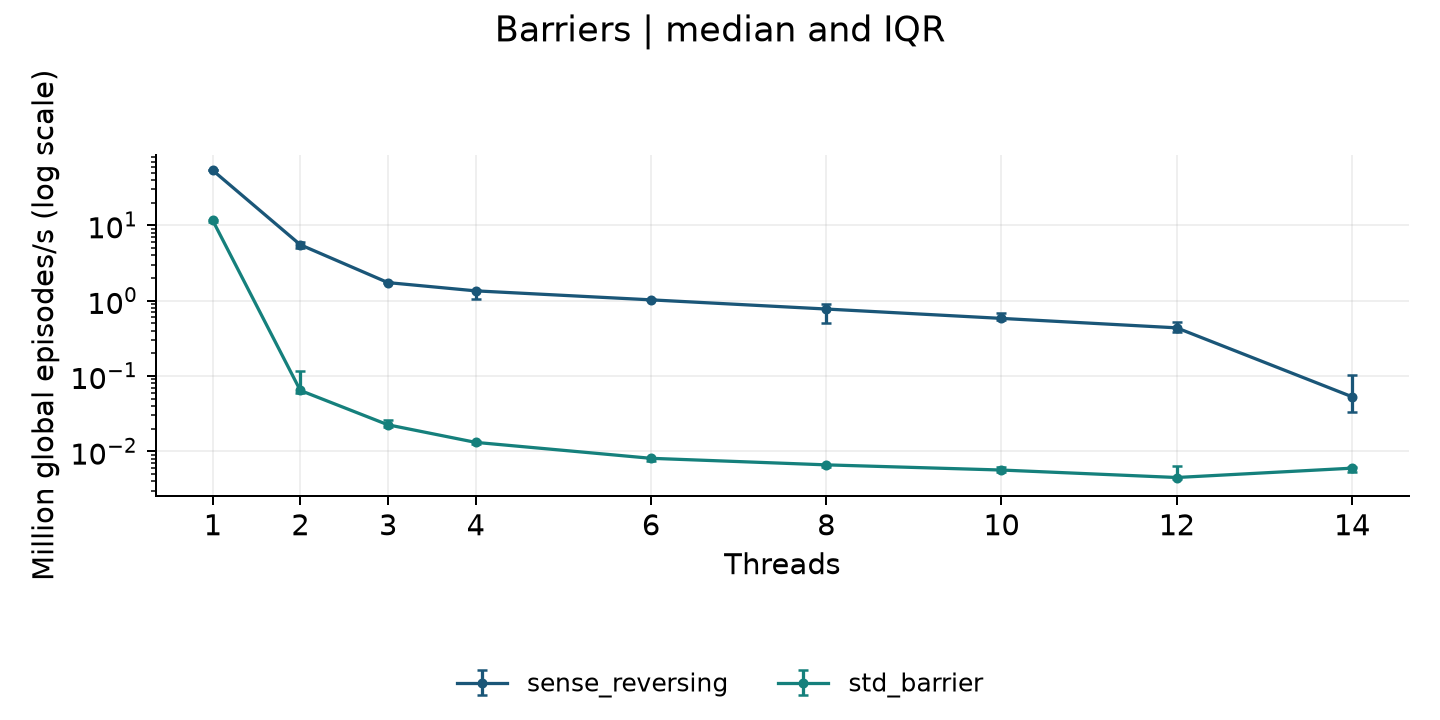
\includegraphics[width=0.85\textwidth]{figures/barriers.png}
\caption{Global barrier episodes per second, $E=20000$, no work between episodes (log scale).}\label{fig:barriers}
\end{figure}

\begin{table}[H]
\centering
\footnotesize
\setlength{\tabcolsep}{3pt}
\caption{Median global barrier episodes per second (thousands), $E=20000$, no work between episodes. Bold: highest at each $P$.}\label{tab:barriers}
\begin{tabular}{|>{\raggedright\arraybackslash}p{\dimexpr 0.200\textwidth-2\tabcolsep-\arrayrulewidth\relax}|>{\raggedleft\arraybackslash}p{\dimexpr 0.088\textwidth-2\tabcolsep-\arrayrulewidth\relax}|>{\raggedleft\arraybackslash}p{\dimexpr 0.088\textwidth-2\tabcolsep-\arrayrulewidth\relax}|>{\raggedleft\arraybackslash}p{\dimexpr 0.088\textwidth-2\tabcolsep-\arrayrulewidth\relax}|>{\raggedleft\arraybackslash}p{\dimexpr 0.088\textwidth-2\tabcolsep-\arrayrulewidth\relax}|>{\raggedleft\arraybackslash}p{\dimexpr 0.088\textwidth-2\tabcolsep-\arrayrulewidth\relax}|>{\raggedleft\arraybackslash}p{\dimexpr 0.088\textwidth-2\tabcolsep-\arrayrulewidth\relax}|>{\raggedleft\arraybackslash}p{\dimexpr 0.088\textwidth-2\tabcolsep-\arrayrulewidth\relax}|>{\raggedleft\arraybackslash}p{\dimexpr 0.088\textwidth-2\tabcolsep-\arrayrulewidth\relax}|>{\raggedleft\arraybackslash}p{\dimexpr 0.088\textwidth-2\tabcolsep-\arrayrulewidth\relax}|}
\hline
\textbf{Barrier (k/s)} & \textbf{P=1} & \textbf{P=2} & \textbf{P=3} & \textbf{P=4} & \textbf{P=6} & \textbf{P=8} & \textbf{P=10} & \textbf{P=12} & \textbf{P=14} \\ \hline
\texttt{sense\_reversing} & \textbf{53\,648} & \textbf{5\,510.2} & \textbf{1\,734.2} & \textbf{1\,348.0} & \textbf{1\,024.0} & \textbf{773.6} & \textbf{581.0} & \textbf{435.2} & \textbf{53.0} \\ \hline
\texttt{std\_barrier} & 11\,634 & 64.3 & 22.5 & 13.1 & 8.1 & 6.6 & 5.6 & 4.5 & 6.0 \\ \hline
\end{tabular}
\end{table}


At $P=1$ a barrier synchronizes nothing, so 54 million episodes per second only measure the cost of one call. From $P=2$ on, the sense-reversing barrier completes 5.5 million episodes per second against 64 thousand for \texttt{std::barrier}, and 435 thousand against 4.5 thousand at $P=12$: about two orders of magnitude. The sense-reversing barrier releases all waiters with one store to the sense flag, which each waiter sees in its spinning load. \texttt{std::barrier} in the GNU implementation is designed to let a waiting thread block after a short spin, so an episode can include operating-system wake-ups; its rate, nearly flat at 4.5--6.6 thousand per second from $P=8$ to 16, is consistent with a wake-up-bound cost.

The rate of the sense-reversing barrier falls as $P$ grows, because all arrivals perform an RMW on the same counter and the last thread must reach the barrier before anyone leaves. At $P=14$ it drops to 53 thousand per second in the main run and 127 thousand in the saturation run (Table~\ref{tab:saturation-barriers}), and to 22 thousand at $P=16$, still 3.7 times faster than \texttt{std::barrier}. A busy-waiting barrier depends on every participant running: one preempted thread stalls the whole episode. The difference between the two runs at $P=14$ shows how sensitive this regime is to the scheduler.

\begin{table}[H]
\centering
\footnotesize
\setlength{\tabcolsep}{3pt}
\caption{Saturation run: median global episodes per second (thousands). Bold: highest at each $P$.}\label{tab:saturation-barriers}
\begin{tabular}{|>{\raggedright\arraybackslash}p{\dimexpr 0.200\textwidth-2\tabcolsep-\arrayrulewidth\relax}|>{\raggedleft\arraybackslash}p{\dimexpr 0.199\textwidth-2\tabcolsep-\arrayrulewidth\relax}|>{\raggedleft\arraybackslash}p{\dimexpr 0.199\textwidth-2\tabcolsep-\arrayrulewidth\relax}|>{\raggedleft\arraybackslash}p{\dimexpr 0.199\textwidth-2\tabcolsep-\arrayrulewidth\relax}|>{\raggedleft\arraybackslash}p{\dimexpr 0.199\textwidth-2\tabcolsep-\arrayrulewidth\relax}|}
\hline
\textbf{Barrier (k/s)} & \textbf{P=12} & \textbf{P=14} & \textbf{P=15} & \textbf{P=16} \\ \hline
\texttt{sense\_reversing} & \textbf{426.3} & \textbf{127.4} & \textbf{112.6} & \textbf{22.3} \\ \hline
\texttt{std\_barrier} & 6.2 & 6.1 & 6.0 & 6.1 \\ \hline
\end{tabular}
\end{table}


\subsection{Concurrent counters}\label{sec:res-counters}

Figure~\ref{fig:counters} and Table~\ref{tab:counters} show the time for $K=1000000$ increments in total.

\begin{figure}[H]
\centering
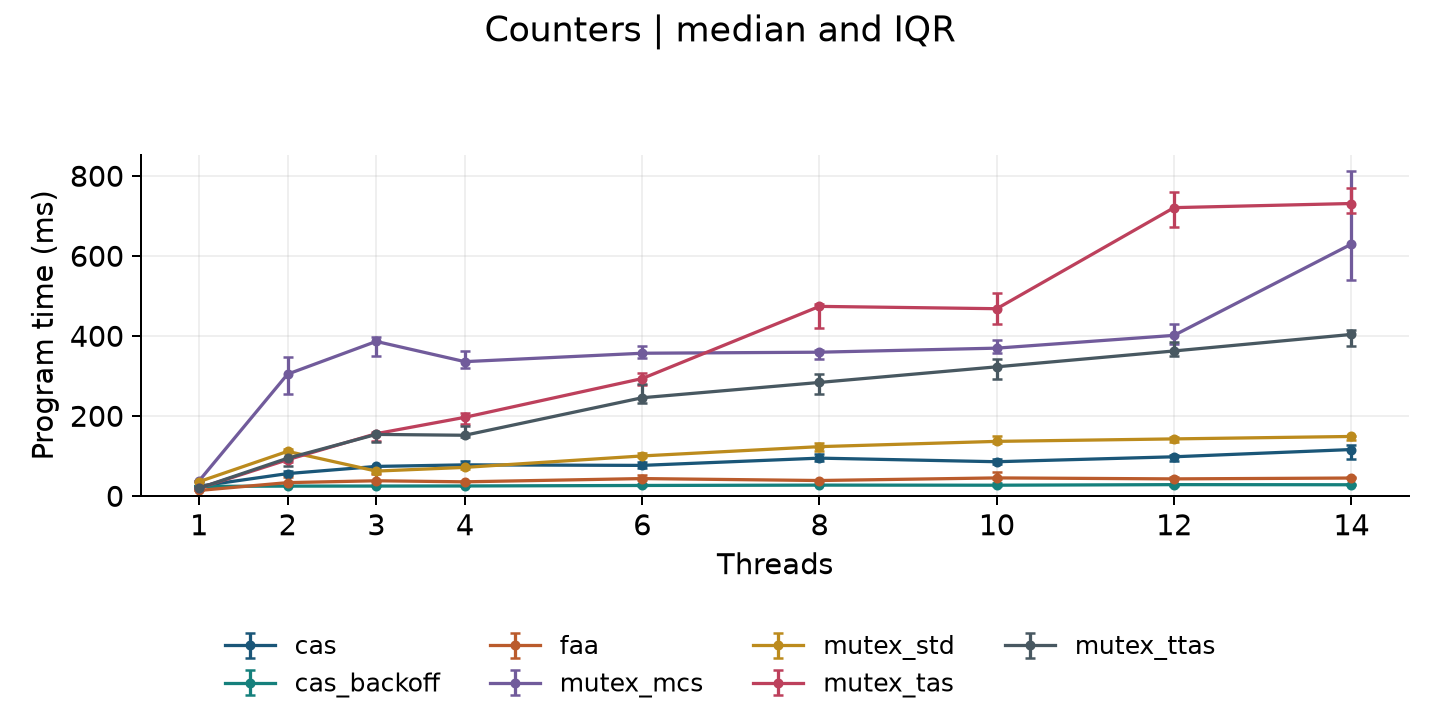
\includegraphics[width=0.85\textwidth]{figures/counters.png}
\caption{Counter program time for $K=1000000$ increments in total (median and IQR).}\label{fig:counters}
\end{figure}

\begin{table}[H]
\centering
\footnotesize
\setlength{\tabcolsep}{3pt}
\caption{Median program time (ms) for $K=1000000$ increments in total. Bold: fastest at each $P$.}\label{tab:counters}
\begin{tabular}{|>{\raggedright\arraybackslash}p{\dimexpr 0.200\textwidth-2\tabcolsep-\arrayrulewidth\relax}|>{\raggedleft\arraybackslash}p{\dimexpr 0.088\textwidth-2\tabcolsep-\arrayrulewidth\relax}|>{\raggedleft\arraybackslash}p{\dimexpr 0.088\textwidth-2\tabcolsep-\arrayrulewidth\relax}|>{\raggedleft\arraybackslash}p{\dimexpr 0.088\textwidth-2\tabcolsep-\arrayrulewidth\relax}|>{\raggedleft\arraybackslash}p{\dimexpr 0.088\textwidth-2\tabcolsep-\arrayrulewidth\relax}|>{\raggedleft\arraybackslash}p{\dimexpr 0.088\textwidth-2\tabcolsep-\arrayrulewidth\relax}|>{\raggedleft\arraybackslash}p{\dimexpr 0.088\textwidth-2\tabcolsep-\arrayrulewidth\relax}|>{\raggedleft\arraybackslash}p{\dimexpr 0.088\textwidth-2\tabcolsep-\arrayrulewidth\relax}|>{\raggedleft\arraybackslash}p{\dimexpr 0.088\textwidth-2\tabcolsep-\arrayrulewidth\relax}|>{\raggedleft\arraybackslash}p{\dimexpr 0.088\textwidth-2\tabcolsep-\arrayrulewidth\relax}|}
\hline
\textbf{Counter (ms)} & \textbf{P=1} & \textbf{P=2} & \textbf{P=3} & \textbf{P=4} & \textbf{P=6} & \textbf{P=8} & \textbf{P=10} & \textbf{P=12} & \textbf{P=14} \\ \hline
\texttt{mutex\_tas} & 19.5 & 90.5 & 155.6 & 196.6 & 293.4 & 473.8 & 468.0 & 720.6 & 731.0 \\ \hline
\texttt{mutex\_ttas} & 19.4 & 94.3 & 153.8 & 151.7 & 245.5 & 283.7 & 322.8 & 362.4 & 403.7 \\ \hline
\texttt{mutex\_mcs} & 37.3 & 304.4 & 386.3 & 335.7 & 356.7 & 359.3 & 369.4 & 401.4 & 629.4 \\ \hline
\texttt{mutex\_std} & 35.6 & 111.4 & 62.1 & 71.4 & 100.0 & 123.2 & 136.4 & 142.6 & 148.7 \\ \hline
\texttt{cas} & 24.4 & 55.9 & 73.8 & 77.7 & 76.4 & 94.5 & 85.5 & 97.9 & 116.0 \\ \hline
\texttt{cas\_backoff} & 23.9 & \textbf{24.6} & \textbf{24.8} & \textbf{24.9} & \textbf{26.2} & \textbf{27.1} & \textbf{26.9} & \textbf{28.3} & \textbf{28.0} \\ \hline
\texttt{faa} & \textbf{13.7} & 33.3 & 37.9 & 35.3 & 43.4 & 38.6 & 45.1 & 42.7 & 44.8 \\ \hline
\end{tabular}
\end{table}


\textbf{No counter is faster with more threads.} The fastest result is FAA with one thread, 13.7~ms. Every increment must update the same cache line, so the increments are serialized in hardware whatever the algorithm, and with more threads the line also moves between cores on every increment. A shared counter is a serial bottleneck, not a parallel workload.

\textbf{CAS with backoff} stays at 24--28~ms for every $P$, the lowest time from $P=2$ on. After a failed CAS the losing threads pause, so the winner can complete many increments in a row while its core owns the cache line. This raises throughput but concentrates the work on one thread at a time; it does not make the counter fairer. \textbf{Plain CAS} rises from 24~ms to 116~ms at $P=14$, because every failed attempt still moves the line. \textbf{FAA} stays at 33--45~ms for $P\ge2$, since an increment is a single RMW that cannot fail.

\textbf{Lock-based counters} pay an acquire and a release per increment, and the critical section is a single addition, so the cost of passing the lock dominates. With $P=14$ the counter takes 149~ms with \texttt{std::mutex}, 404~ms with TTAS, 629~ms with MCS and 731~ms with TAS. MCS is already at 304~ms with two threads, against 37~ms with one, presumably because almost every increment then hands the lock to a thread on another core. The ranking also differs from the prime workload: with $W=0$ at $P=14$, TAS beats \texttt{std::mutex} (108 against 122~ms), but in the counter, whose critical section is a single addition, TAS is the slowest lock and \texttt{std::mutex} the fastest. A lock cannot be chosen without knowing the length of the critical section and the number of threads.

\subsection{Summary of findings}

\begin{table}[H]
\centering
\small
\caption{Main findings on the measured laptop.}\label{tab:findings}
\begin{tabular}{|>{\raggedright\arraybackslash}p{\dimexpr 0.25\textwidth-2\tabcolsep-\arrayrulewidth\relax}|>{\raggedright\arraybackslash}p{\dimexpr 0.745\textwidth-2\tabcolsep-\arrayrulewidth\relax}|}
\hline
\textbf{Topic} & \textbf{Finding} \\ \hline
Speedup bound & Spinlocks reach 1.9$\times$, 2.8$\times$, 3.9$\times$ and 5.6$\times$ for $W=1,2,4,8$, against Amdahl bounds of 2, 3, 5 and 9. \\ \hline
TAS vs.\ TTAS & TTAS's read-only waiting matters with frequent handoffs: 106 against 244~ms at $P=14$, $N=97$. \\ \hline
MCS & Competitive up to about 10 threads; collapses at $P=15$--16 because a preempted queue successor blocks the lock. \\ \hline
\texttt{std::mutex} & A constant handoff cost of about 34\% over the serial bound; slower than one thread at $W=1$; robust when threads exceed CPUs. \\ \hline
Backoff & Modest gains for TTAS; large gains for the CAS counter, by serializing the work. \\ \hline
Barrier & Sense reversal is about 100$\times$ faster than \texttt{std::barrier} up to 12 threads and still 3.7$\times$ at 16. \\ \hline
Counters & No variant scales; FAA is the fastest single-thread option, CAS with backoff the fastest multi-thread option. \\ \hline
\end{tabular}
\end{table}
